\chapter{Обзор технологий организации вычислительных сетей}

\section{Определение локальных сетей}

Локальными сетями называют частные сети, размещающиеся, как правило, в одном здании или
на территории какой-либо организации. Их часто используют для объединения компьютеров и
рабочих станций в офисах компании или предприятия бытовой электроники для предоставления
совместного доступа к ресурсам (например, принтерам) и обмена информацией
\cite{tanenbaum}. Важными требованими, предъявляемыми к ЛВС, являются:

\begin{itemize}
    \item Низкий уровень ошибок передачи, вызванных внутренними или внешними факторами.
        Допустимая вероятность ошибок передачи данных должна быть порядка
        $10^{-8}$–$10^{-12}$.
    
    \item Возможность  работы  с  большими нагрузками  или высокая интенсивность обмена.
        Если механизм управления в сети не эффективен, то компьютеры могут подолгу ждать
        свою очередь на передачу. И даже если передача будет на высочайшей высоте и
        безошибочна, задержка доступа пользователю данной сети будет неприемлема.
\end{itemize}

Большинство ЛВС имеет выход в глобальную сеть. Но характер информации,  принципы
организации  обмена,  режимы  доступа  к  ресурсам внутри (ЛВС), как правило, отличаются
от принципов, принятых в глобальной сети. Возможность выхода в глобальную сеть — это
лишь один из ресурсов, разделяемых пользователями ЛВС. По ЛВС могут передаваться:
данные, изображения, телефонные разговоры, электронные письма и т.д. Чаще всего ЛВС
используются для совместного использования дискового пространства, принтеров и факсов,
выхода в глобальную сеть, но это лишь часть тех возможностей, которые предоставляют ЛВС. 

Например,  они  позволяют  осуществлять  обмен  информацией между
компьютерами  разных типов. ЛВС дают возможность организовать систему параллельных
вычислений на всех компьютерах сети, что ускоряет решение сложных задач. С их помощью,
можно управлять работой техноло-гической системы или исследовательской установки с
нескольких компью-теров одновременно. Однако ЛВС имеют ряд существенных недостатков:

\begin{itemize}
    \item ЛВС требует дополнительных, иногда значительных материальных затрат на
        покупку сетевого оборудования, ПО, на прокладку кабелей и обучение персонала. 
    \item ЛВС требует приема на работу специалиста (администратора сети),  который
        будет контролировать  работу сети, модернизировать, управлять доступом к
        ресурсам, устранять возможные неисправности, защищать информацию и делать
        резервные копии. Для больших сетей может понадобиться целая бригада
        специалистов. ЛВС ограничивает перемещение компьютеров, подключенных к ней, так
        как при этом требуется перекладка соединительных кабелей.
    \item ЛВС являются прекрасной средой для распространения компьютерных  вирусов,
        поэтому придется уделять  много  времени  вопросу о защите от них. Все
        компьютеры сети могут быть заражены, если заразить всего один.
    \item ЛВС резко повышают опасность несанкционированного доступа к информации с целью
        ее кражи или уничтожения. Информационная защита требует проведения комплекса
        технических и организационных мероприятий.
\end{itemize}

ЛВС классифицируются,  прежде  всего, по протоколам  1-го  и  2-го уровней OSI, то есть,
по технологии используемого сетевого оборудования: Ethernet, Token Ring, FDDI,
AppleTalk. По масштабам и иерархии построения ЛВС различают: 
\begin{itemize}
    \item сети рабочих групп (5-20 станций); 
    \item сети отделов (20-100 станций); 
    \item сети предприятий (корпоративные сети).
\end{itemize}

Последние имеют  развернутую структуру  сетевых  служб  и  по  географии могут выходить
за рамки локальных сетей, образуя кампусные сети, сети с удаленным доступом, а также
сети других масштабов, вплоть до корпоративных частных глобальных сетей. Количество
станций в корпоративных сетях варьируется: от 20 компьютеров до десятков тысяч.

\begin{figure}[h]
    \center
    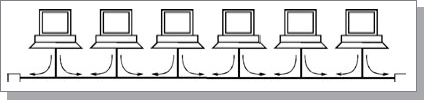
\includegraphics[width=0.7\linewidth]{topo_bus}
    \caption{Топология {шина}}
    \label{pic:topo_bus}
\end{figure}
\begin{figure}[h]
    \center
    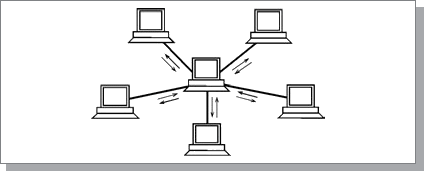
\includegraphics[width=0.7\linewidth]{topo_star}
    \caption{Топология {звезда}}
    \label{pic:topo_star}
\end{figure}
\begin{figure}[h]
    \center
    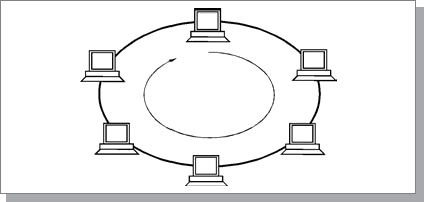
\includegraphics[width=0.7\linewidth]{topo_ring}
    \caption{Топология {кольцо}}
    \label{pic:topo_ring}
\end{figure}

Для организации сетей используются различные топологии. Основных топологии, применяемые
в ЛВС, такие: 

Шина (bus) — все устройства параллельно подключаются к одной линии связи. Информация
от каждого устройства одновременно передается всем остальным
(см. рисунок \ref{pic:topo_bus}).

Звезда (star) — к одному центральному устройству присоединяются остальные периферийные
устройства, причем каждый из них использует отдельную линию связи. Информация
от периферийного устройства направляется только центральному, а от него —
одному или нескольким периферийным
(см. рисунок \ref{pic:topo_star}).

Кольцо (ring) — устройства последовательно объединены в кольцо. Передача информации
в кольце всегда производится только в одном направлении. Каждое из устройств
передает информацию только одному следующему в цепочке за ним, а
получает информацию только от предыдущего в цепочке.
(см. рисунок \ref{pic:topo_ring}).

В зависимости от характера распределения функций различают: 

\begin{itemize}
    \item одноранговые  сети — небольшие  локальные  сети,  в которых компьютеры являются
        равноправными; обычно включают в себя до 15 станций;

    \item сети с выделенными серверами (двухранговые сети) — средние и крупные сети, в
        которых часть выполняемых функций обслуживания станций возложена на серверы. Такие
        сети характеризуются типами  используемых в них сетевых служб: файловая служба,
        служба печати, служба терминалов, управление базами данных, Web-служба, почтовая
        служба, службы интерактивного общения, прокси-сервер, сетевая безопасность.
\end{itemize}

